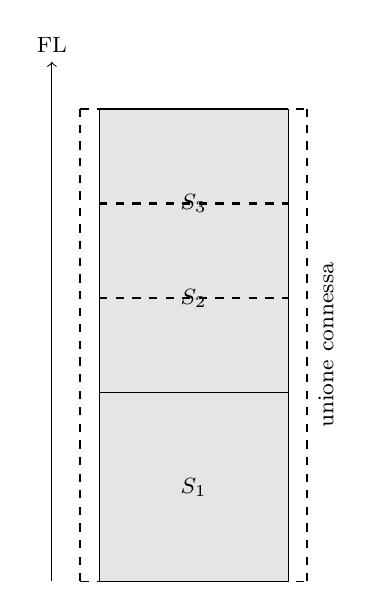
\begin{tikzpicture}[scale=1.2, font=\footnotesize]
  \draw[->] (0,0) -- (0,5.5) node[above] {FL};

  \draw[fill=gray!20] (0.5,0) rectangle (2.5,2);
  \node at (1.5,1) {$S_1$};

  \draw[fill=gray!20] (0.5,2) rectangle (2.5,4);
  \draw[fill=gray!20, draw=none] (0.5,3) rectangle (2.5,5); % Solo riempimento
  \draw (0.5,3) -- (0.5,5); % lato sinistro
  \draw (0.5,5) -- (2.5,5); % lato superiore
  \draw (2.5,5) -- (2.5,3); % lato destro
  \node at (1.5,4) {$S_3$};
  \node at (1.5,3) {$S_2$};

  
  \draw[dashed,thick] (0.5,4)--(2.5,4);
  \draw[dashed,thick] (0.5,3)--(2.5,3);
  \draw[dashed,thick] (0.3,0)--(0.3,5);
  \draw[dashed,thick] (2.7,0)--(2.7,5);
  \draw[dashed]      (0.3,0)--(2.7,0);
  \draw[dashed]      (0.3,5)--(2.7,5);
  \node[rotate=90] at (2.9,2.5) {unione connessa};
\end{tikzpicture}